\section{METHOD}
\chadded[id=zheliku]{
  A VR twin is a fundamental interaction unit comprising a Real Interactive Object (RIO) in the physical world and its corresponding Virtual Interactive Object (VIO) in the virtual environment. The VIO provides visual feedback, while the RIO delivers haptic feedback. Crucially, VR twins enable users to interact through natural hand gestures without additional learning costs. Users perceive realistic haptic feedback during virtual interactions, mirroring the experience of manipulating real-world objects.
}

\subsection{Data Synchronization}
The VIO of VR twin synchronize the state (e.g., position, angle) of their corresponding RIO. Data communication between them is achieved through real-time sensing technology. Each of the three VR twins is equipped with specific sensors to capture the physical properties of the RIO, which is then filtered and transmitted to the VIO via Arduino for real-time updates.

\subsubsection{Sensing Solution}
Each RIO is instrumented with application-specific sensors to capture its physical state and user inputs. Key considerations include:
\begin{enumerate}
  \item Sensor Selection: Based on the interaction modality (e.g., linear displacement, rotary motion, pressure application), appropriate sensors (e.g., tension/load cells, accelerometers, gyroscopes, pressure sensors, rotary encoders, potentiometers) are integrated.

  \item Performance Specification: Sensors are characterized by their operating frequency, measurement range, resolution, and accuracy, tailored to the required fidelity and dynamics of the interaction. Common parameters include sampling rates (e.g., 50-100 Hz), force ranges (e.g., 0-20 $N$), displacement/angle resolutions (e.g., 0.01 $m/s^2$, 0.5$^\circ$), and pressure resolutions (e.g., 0.01 $N$).
\end{enumerate}

\subsubsection{Data Communication}
A robust communication architecture ensures low-latency data transfer between RIOs and the host system (e.g., PC running the VR environment):

\begin{enumerate}
  \item Hardware Platform: Microcontrollers (e.g., Arduino UNO) serve as the interface, acquiring raw sensor data. Signal conditioning modules (e.g., HX711 for high-gain amplification and 24-bit ADC) are employed for precision analog measurements.

  \item System Architecture: A distributed architecture is often advantageous. Each RIO (or sensor group) connects to a dedicated microcontroller, enabling parallel data acquisition. These microcontrollers communicate with the host via independent serial links (e.g., USB virtual COM ports).
  
  \item Host-Side Handling: The host system implements multi-port communication to concurrently monitor data streams from all RIOs. Data packets are parsed using predefined identifiers (device ID, sensor type) to extract and structure measurements for subsequent processing.
\end{enumerate}

\subsubsection{Data Processing}
Raw sensor data undergoes a pipeline of processing steps to enhance signal quality, normalize inputs, and derive meaningful interaction states:

\begin{enumerate}
  \item \texttt{Noise Reduction}: Kalman filtering is applied to raw data to estimate the true system state by optimally combining predictions and noisy measurements, significantly reducing environmental and sensor noise impact.

  \item \texttt{Input Normalization}: Sensor readings are normalized to a consistent range (e.g., [0, 1]) relative to predefined operational limits. The lower limit typically corresponds to the RIO's initial/rest state. The upper limit is determined empirically (e.g., via repeated user trials capturing maximum expected input values) or based on sensor specifications.

  \item \texttt{State Detection \& Smoothing}: Processed/normalized data ($x_t$ at time $t$) is used to determine interaction states and smooth transitions:
  
  \begin{enumerate}
    \item Thresholding: State changes (e.g., engagement, disengagement) are detected using empirically derived thresholds (e.g., $x_t > 0.05$).

    \item Change Detection: Significant changes ($Δx_t >$ threshold) indicate state transitions (e.g., object release/return).

    \item Interpolation: Techniques like linear interpolation are applied to $x_t$ to ensure smooth visual updates of the VIO's state (position, rotation) in the virtual environment.
  \end{enumerate}

\end{enumerate}

\subsection{Virtual-Real Alignment}
Virtual-Real Alignment ensures precise spatial correspondence and consistent interactive behavior between the VIO and its RIO counterpart. This is paramount for delivering authentic and synchronized visual and haptic feedback, thereby maximizing user immersion and interaction fidelity.

\subsubsection{Spaital Alignment}
RIOs are mounted in a fixed spatial relationship, often on a stable platform, establishing a reliable physical reference frame. The virtual scene is constructed using a defined scale ratio between virtual units (e.g., Unity units) and real-world units (e.g., meters). VIOs are scaled and positioned within the virtual environment to exactly match the relative positions and orientations of their RIOs in the physical reference frame. Processed RIO sensor data ($x_t$) is continuously mapped to control the VIO's state:
\begin{enumerate}
  \item For linear interactions, $x_t$ drives displacement along defined axes (e.g., position = $x_t \times$ max\_displacement).

  \item For angular interactions, $x_t$ directly controls rotation.

  \item For binary or ranged states (e.g., pressed/released), $x_t$ interpolates between defined states (e.g., height = max\_height - (max\_height - min\_height) $\times x_t$).
\end{enumerate}


\subsubsection{Interaction Calibration}
Achieving robust interaction requires mitigating inherent inaccuracies in gesture tracking that can cause visual artifacts like virtual hand penetration into VIOs (Fig. \ref{fig:gesture-tracking-deviations-b}) or unrealistic object motion if simulated physics are applied (Fig. \ref{fig:gesture-tracking-deviations-c}). Our solution employs a three-pronged approach:

\begin{figure}
  \begin{subfigure}{0.31\linewidth} % 子图 (a)
    \centering
    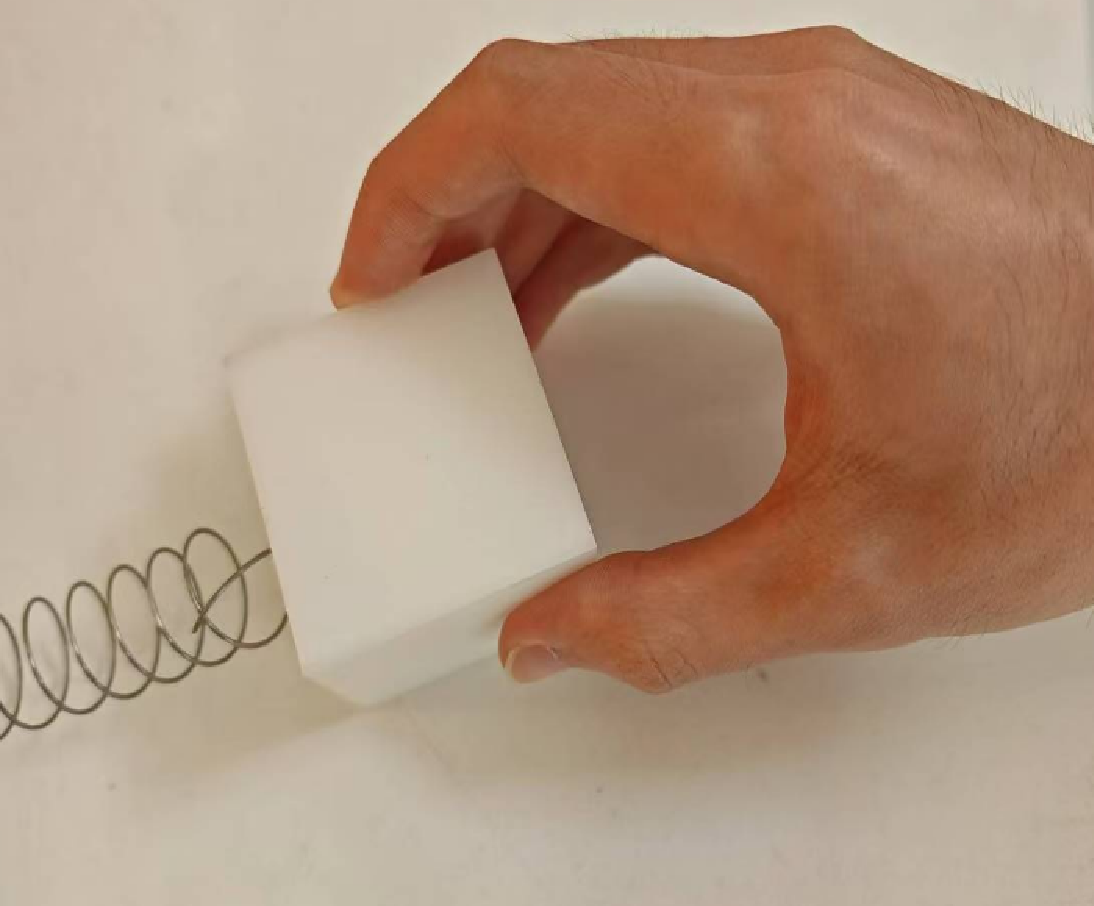
\includegraphics[width=\linewidth]{image/gesture-tracking-deviations-a.pdf}
    \caption{} % 子图标题 (a) 的内容
    \label{fig:gesture-tracking-deviations-a}
  \end{subfigure}
  \hfill % 水平填充间隔
  \begin{subfigure}{0.31\linewidth} % 子图 (b)
    \centering
    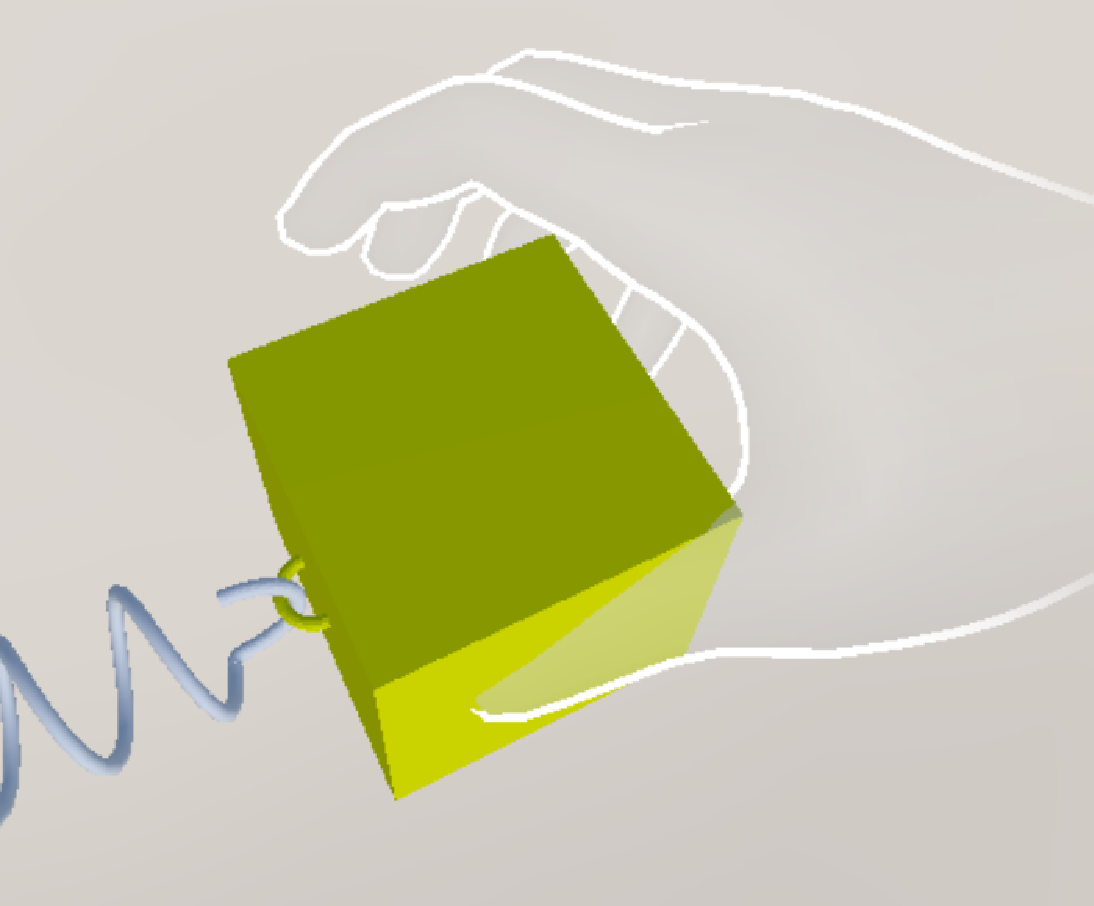
\includegraphics[width=\linewidth]{image/gesture-tracking-deviations-b.pdf}
    \caption{} % 子图标题 (b) 的内容
    \label{fig:gesture-tracking-deviations-b}
  \end{subfigure}
  \hfill % 水平填充间隔
  \begin{subfigure}{0.31\linewidth} % 子图 (c)
    \centering
    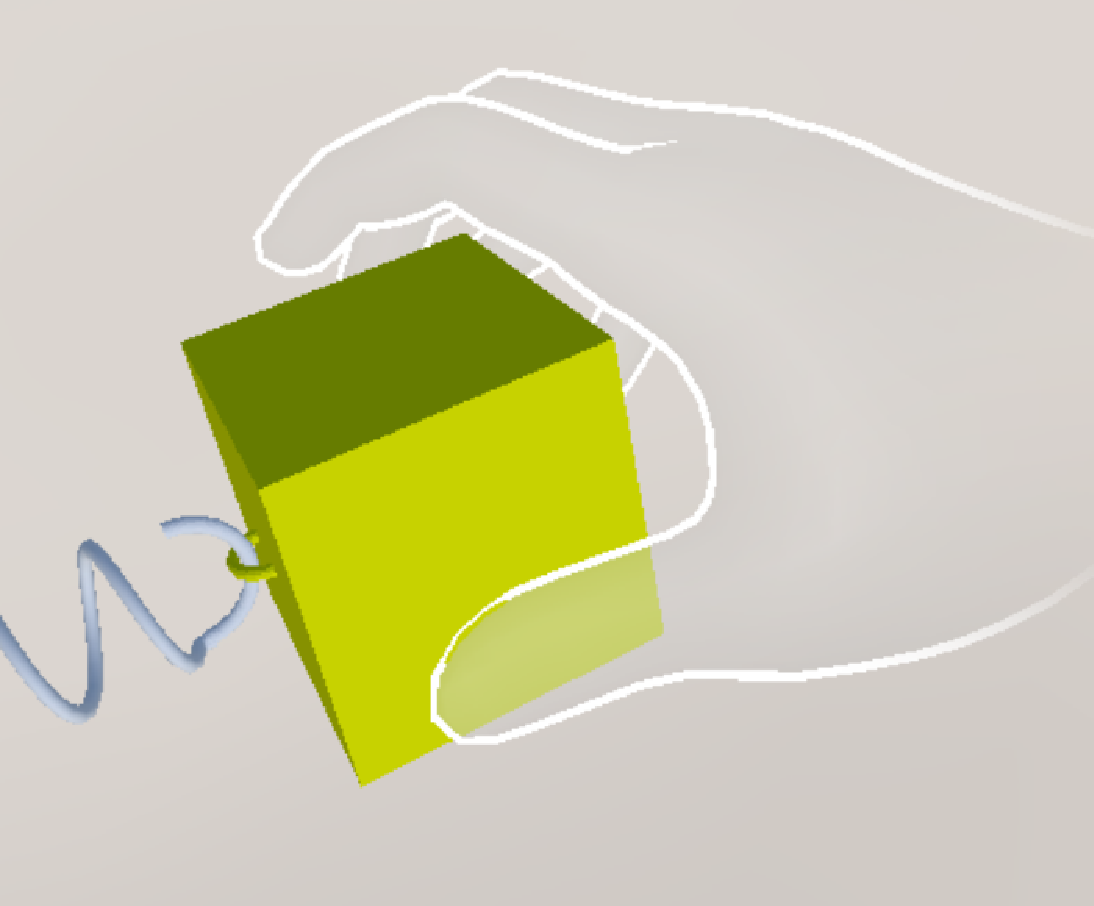
\includegraphics[width=\linewidth]{image/gesture-tracking-deviations-c.pdf}
    \caption{} % 子图标题 (c) 的内容
    \label{fig:gesture-tracking-deviations-c}
  \end{subfigure}
  \caption{Misalignment issue in gesture tracking. (\subref{fig:gesture-tracking-deviations-a}) Real interaction, (\subref{fig:gesture-tracking-deviations-b}) Virtual hand penetration, (\subref{fig:gesture-tracking-deviations-c}) Irregular object motion.}
  \label{fig:gesture-tracking-deviations}
\end{figure}


\paragraph{VIO Motion Independence}: The VIO's core motion (position, rotation) is solely driven by RIO sensor data. The VIO is assigned infinite mass within the physics engine, ensuring it remains unaffected by unintended virtual hand collisions, preventing unnatural jitter or displacement.

\paragraph{Gesture Parameterization \& Predefinition}: Hand gesture characteristics (joint positions, finger lengths, bending angles) are parameterized. For each VIO type, interaction-specific canonical gestures are predefined, optimized to match the VIO's geometry and intended manipulation method. Examples include a semi-closed grasp for cylindrical objects or an extended finger pose for button pressing.

\paragraph{Dynamic Collision Handling via Gesture Prediction}:
\begin{enumerate}
  \item Interaction Trigger Zone: A spherical bounding volume centered on the user's virtual palm defines the proximity region for potential interaction initiation (Fig. \ref{fig:bounding-volume}).
  \item Hand Collision Model: A simplified sphere tree model approximates the collision geometry of the virtual hand (e.g., spheres at key joints and palm) (Fig. \ref{fig:sphere-tree-model}).

  \begin{figure}
    \begin{subfigure}{0.48\linewidth} % 子图 (a)
      \centering
      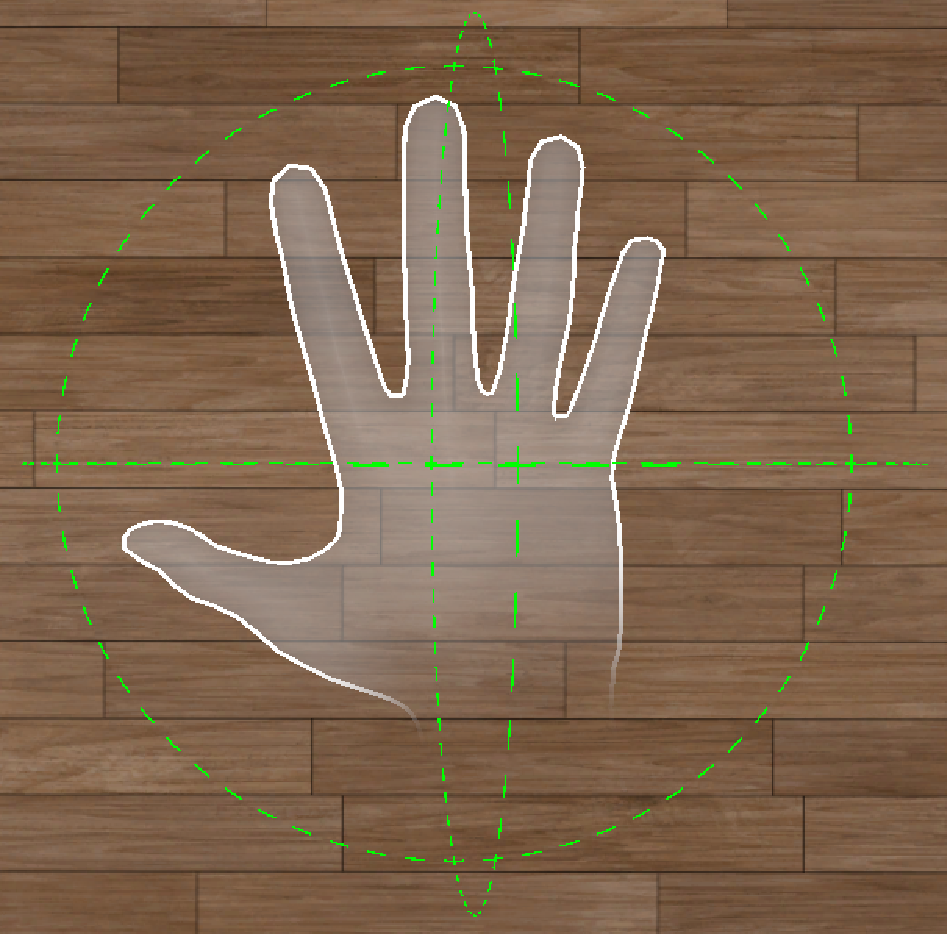
\includegraphics[width=\linewidth]{image/bounding-volume.pdf}
      \caption{} % 子图标题 (a) 的内容
      \label{fig:bounding-volume}
    \end{subfigure}
    \hfill % 水平填充间隔
    \begin{subfigure}{0.48\linewidth} % 子图 (b)
      \centering
      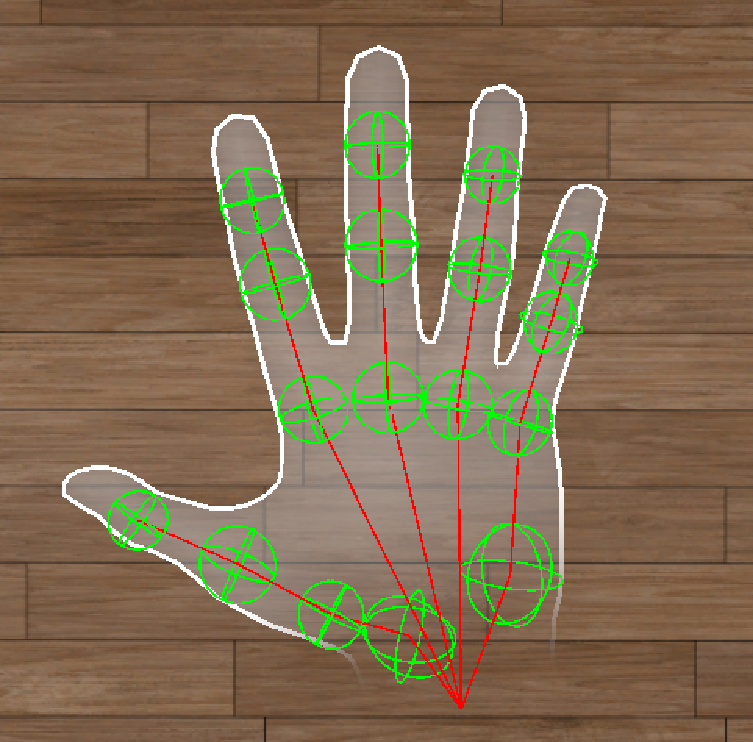
\includegraphics[width=\linewidth]{image/sphere-tree-model.pdf}
      \caption{} % 子图标题 (b) 的内容
      \label{fig:sphere-tree-model}
    \end{subfigure}
    \caption{Bounding volume and sphere tree model for the virtual hand. (\subref{fig:bounding-volume}) Spherical bounding volume, (\subref{fig:sphere-tree-model}) Sphere tree model.}
    \label{fig:bounding-volume-and-sphere-tree-model}
  \end{figure}

  \item State-Based Collision Strategy:
    \begin{enumerate}
      \item Interacting State: When the hand enters the trigger zone and the user's tracked gesture sufficiently matches the VIO's predefined interaction gesture, the system initiates the interaction: 
      \begin{enumerate}
        \item The virtual hand smoothly interpolates towards the predefined canonical pose to minimize visual penetration. \item Physics-based collision between the hand's sphere tree and the VIO is disabled to prevent penetration artifacts while the interaction gesture is active.
      \end{enumerate}

      \item Non-Interacting State: Outside the trigger zone or without a matching gesture: 
      \begin{enumerate}
        \item Physics-based collision using the hand's sphere tree is enabled. 
        \item This prevents the virtual hand from passing through the VIO. 
        \item Due to the VIO's infinite mass, collisions do not cause unrealistic VIO motion, only constraining the hand's position.
      \end{enumerate}
  \end{enumerate}

\end{enumerate}